\chapter{Conclusiones y trabajo futuro}
\label{ch:chap06}

Este capítulo presenta las conclusiones principales en relación a la investigación realizada sobre el modelo de iluminación global implementado y sus extensiones para considerar superficies especulares, junto a un conjunto de posibles líneas de trabajo para extender los algoritmos implementados.

\section{Conclusiones}
\label{sec:conclusiones}

Este proyecto se dedicó al estudio, adaptación, implementación, extensión y comparación de distintos modelos de iluminación global que han surgido durante los años basados el método de radiosidad, así como posibles estrategias que optimicen el tiempo de ejecución observado. En este sentido, se logró comprobar que las extensiones del método de radiosidad que toman en consideración el fenómeno de la reflexión especular logran resultados con mayor realismo, observándose un costo adicional de computación despreciable, sobre todo al utilizar la técnica de traza de rayos.

Adicionalmente, se comprobó que el método del hemicubo comúnmente usado en la técnica no presenta buenas características para ser integrado en el cálculo de los factores de forma extendidos. Recurrir a métodos auxiliares para computar las direcciones de rebote son aproximaciones que pueden degradar la calidad de los resultados, tanto en el uso de traza de rayos o dibujado de portales. No obstante, el método se muestra superior en escenas exclusivamente difusas aún cuando no se han implementado estructuras de aceleración para el cálculo.

En lo que refiere a la interfaz de usuario y las funcionalidades auxiliares implementadas se ha podido comprobar que fueron de utilidad para facilitar la ejecución y diseño de las pruebas permitiendo la exportación e importación de los datos obtenidos de forma sencilla y genérica. El uso de formatos estandarizados fue sin lugar a dudas una elección que enriqueció la usabilidad del programa.

Sobre las distintas tecnologías utilizadas se destaca la facilidad de manejo de la geometría en Embree como a su vez la flexibilidad de su uso utilizando bibliotecas de manejo de hilos. Además, se destacan las distintas extensiones de OpenGL que hicieron posible el uso de \textit{compute shaders} para reducir los hemicubos proyectados a filas de la matriz de factores de forma y la simpleza del uso de \textit{geometry shaders} y arreglos de texturas para reducir al mínimo los costos de las mutaciones del estado en lo que respecta de \textit{render targets}.

Finalmente, se destaca el uso de la metodología \textit{Kanban} para el control y seguimiento de requerimientos y tareas. Junto al uso de programación orientada a objetos para abstraer los conceptos y ofrecer una capacidad mayor de re-utilización de componentes y extensión de los métodos. Como por ejemplo, la clase \textit{Pipeline} concebida exclusivamente para superficies difusas utilizando OpenGL, que fue luego extendida de forma tal que se incluyeran métodos de traza de rayos con Embree y extensiones de los algoritmos de cálculo de factores de forma. 

\section{Trabajo futuro}
\label{sec:futuro}

Este proyecto puede ser continuado en distintas líneas de trabajo que fueron surgiendo a lo largo de la implementación y estudio de las soluciones desarrolladas.

En primer lugar, sería de gran interés la adición de estructuras de aceleración en OpenGL como por ejemplo, el uso de \textit{octrees}. Estas estructuras arborescentes permiten el descarte de dibujado de ciertas agrupaciones de primitivas a nivel de CPU y por tanto eliminan el costo del cálculo del algoritmo del Z-Buffer en gran medida [Vazquez y Guarte \cite{Guarte}]. Además, sería beneficioso investigar la posible implementación del \textit{renderer} de OpenGL en la API Vulkan, que ha sido optimizada para minimizar el impacto del controlar de la GPU en la CPU, además provee facilidades que permiten enviar comandos de dibujado desde distintos hilos, lo que disminuiría la necesidad de sincronización entre el controlador de pre-procesamiento (\textit{PreprocessorController}) y el controlador del dispositivo.

Por otro lado, sería beneficioso implementar un \textit{plugin} de los algoritmos implementados para \textit{software} de terceros, como por ejemplo el programa \textit{Blender}, que se ha utilizado para editar los objetos 3D en las escenas de prueba aunque provee de funcionalidades que calculan la iluminación global. Además, como se aprecia en la Figura \ref{img:text} el uso de texturas proporciona detalles visuales que enriquecen la imagen generada, aunque la técnica de radiosidad es utilizada para el cálculo de la iluminación, es decir, es una de las etapas necesarias para generar imágenes fotorealistas.

\begin{figure}[H]
	\centering
	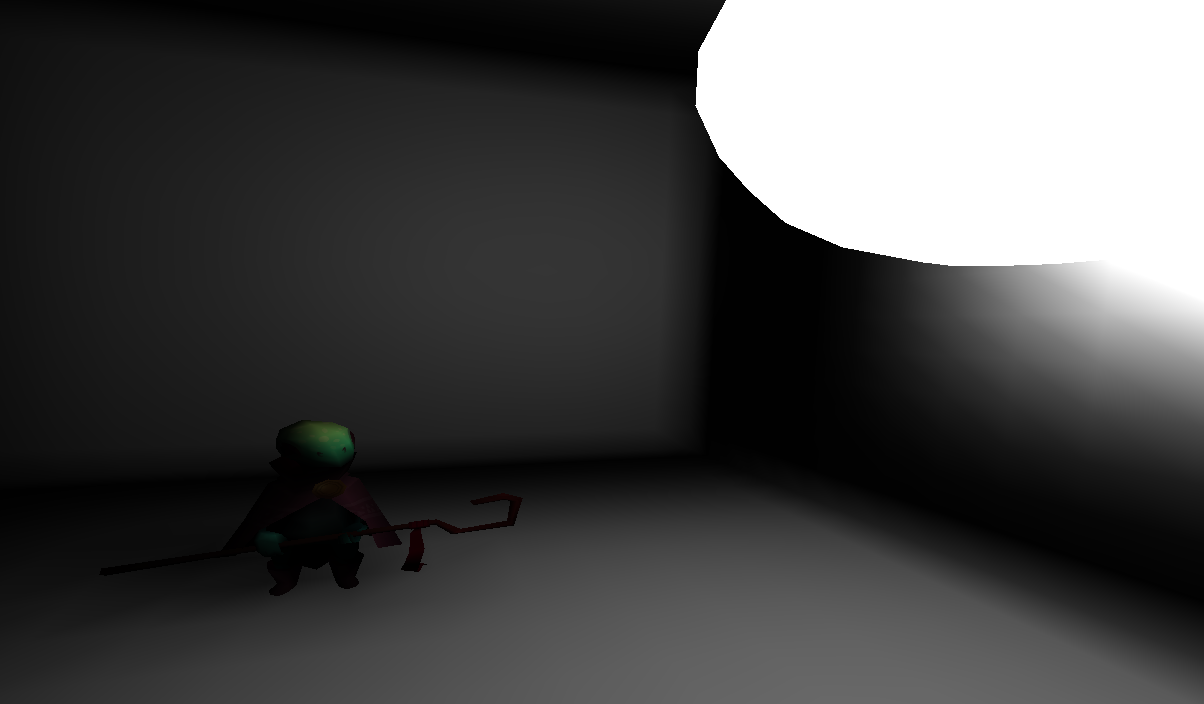
\includegraphics[width=.7\linewidth]{assets/text}
	\caption{Ejemplificación de la adición de texturas a los objetos de la escena}
	\label{img:text}
\end{figure}

Finalmente, el desarrollo de nuevo \textit{hardware} permite la que traza de rayos pueda ser acelerada por la GPU a través de las extensiones DirectX DXR y Vulkan VK\_NVX\_raytracing, que son predominantemente utilizadas con tarjetas gráficas NVIDIA RTX. Por ello se propone el análisis de los algoritmos implementados en este tipo de dispositivos.